\subsection{Deep Learning}\label{subsec:deep-learning}
Deep Learning is a class of machine learning systems whose goal is to extract relevant features from a distribution of data. On an abstract level, Deep Learning systems take inspiration the structure of the human brain, with multi-layer structures of nodes (Neurons): each layer might be thought of as a section of a brain recognizing a very specific element, and when all layers work in unison they can recognize and act upon high level features and categories.

Deep Learning Systems are particularly useful because of their ability to extract high level features from data, especially features that are hard to define algorithmically by humans.

Because of the number of variables involved, it is hard to predict what results might derive from a change in the initial condition; as a consequence of this uncertainty, the process of working with Deep Learning systems is one of incremental change and experimentation. 

Figure \ref{fig:DNN} shows the typical structure of a Deep Neural Network:
\begin{figure}[H]
\centering    
\begin{neuralnetwork}[height=8]
\newcommand{\x}[2]{$x_#2$}
\newcommand{\y}[2]{$y_#2$}
\newcommand{\hfirst}[2]{\small $h1_#2$}
\newcommand{\hsecond}[2]{\small $h2_#2$}
\inputlayer[count=4, bias=false, title=Input Layer, text=\x]
\hiddenlayer[count=8, bias=false, title=Hidden Layer 1, text=\hfirst] \linklayers
\hiddenlayer[count=8, bias=false, title=Hidden Layer 2, text=\hsecond] \linklayers
\outputlayer[count=4, title=Output Layer, text=\y] \linklayers
\end{neuralnetwork}
\caption{An example of a Deep Neural Network}\label{fig:DNN}
\end{figure}
As we can see in the example above, a neural network is composed of an Input Layer, a number of Hidden layers and an Output layer.
Speaking in general terms, the input layer receives a chunk of data to be processed, the hidden layers operate on the input sequentially, and the output layer is where the system expresses a judgement on the data.

The training process for a neural network is composed of two distinct phases: the \emph{Feed Forward} phase and the \emph{Back-Propagation} phase: in the feed forward phase the network processes the current data and comes to a result, then the networks computes the Error (or how much the result it had come to deviated from the expected result).

The network then takes the error value and propagates it backwards by adjusting the weights of the connections between each neuron in the different layers, in an effort to reduce the error. This is the back-propagation phase.
Once both phases are completed, the network has completed an iteration. The next batch of data is then introduced and the process begins anew.

Note that training data is not fed to the network one piece at a time, but instead is introduced in batches. The input data is divided into batches of varying size (64 or 128 samples per batch are common values), and each iteration a new batch of data is loaded into the network; training usually ends once the system runs out of input data.

In the coming sections we will cover two types of Deep Neural Networks that are relevant in this paper: \emph{Recurrent Neural Networks} (RNNs) and  \emph{Generative Adversarial Networks} (GANs).
This following section will cover Recurrent Neural Networks, while section \ref{subsubsec:gans} will cover Generative Adversarial networks: we will explain the structure and operation of GANs in that section, then talk more about PassGAN specifically in section \ref{subsubsec:gans-passgan}.
%\clearpage

\subsubsection{Recurrent Neural Networks}
Recurrent Neural Networks are the simpler of the two network architectures that we will cover: they are a kind of neural network specialized in working with data that has a temporal component.
For instance if the network needs to predict the next letter or word in a sentence, it needs to know what came before. Another example might be a neural network that scales or edits videos, where the action to take on any given frame might be dependent on the frames that came before.

We do not use Recurrent Neural Networks directly in our thesis, but they are used heavily in Melicher et al. \cite{Melicher2016} and we cover them here as an alternative approach to Deep Learning-based password crackers; furthermore they are also relevant in the context of PassGAN, as Hitaj. et al. \cite{PassGAN} compare the performance of PassGAN to the RNN-based system in Melicher et al.

The precise method the network uses to keep track of temporal elements is rather complex, but can be briefly summarized by saying that each neuron in the network holds a state: in each iteration a neuron's state from the previous iteration is fed as input to itself in the current iteration along side the current data to be processed.
This creates a feedback loop, whereby at any given point the calculation performed by each neuron are influenced by previous events.

\begin{figure}[H]    
\centering
\begin{tikzpicture}[shorten >= 1pt, node distance = 2cm, on grid, auto, square/.style={regular polygon, regular polygon sides = 4}]
\node[](0){};
\node[below of = 0](1){};
\node[below of = 1] (2){};

\node[state, right of = 1](N1){$H1_{(t)}$};
\node[state, right of = N1](N2){$H2_{(t)}$};
\node[state, right of = N2](output){$O$};

\draw[-]   (0) edge node{$x_i$} (N1)
            (2) edge node{$x_i$}(N1)
            (N1) edge (N2)
            (N2) edge (output);
\end{tikzpicture}
\begin{center}
Iteration number 1 $t=1$
\end{center}
\end{figure}

\begin{figure}[H]
\centering    
\begin{tikzpicture}[shorten >= 1pt, node distance = 2cm, on grid, auto, square/.style={regular polygon, regular polygon sides = 4}]
	\node[](0){};
	\node[below of = 0](1){};
	\node[below of = 1] (2){};
	
	\node[state, right of = 1](N1){$H1_{(t)}$};
	\node[state, right of = N1](N2){$H2_{(t)}$};
	\node[state, right of = N2](output){$O$};
	
	\draw[-]   (0) edge node{$x_i$}(N1)
	(2) edge node{$x_i$} (N1)
	(N1) edge[loop above] node{$H1_{(t-1)}$} (N1)
	(N2) edge[loop above] node{$H2_{(t-1)}$} (N2)
	(N1) edge (N2)
	(N2) edge (output);	
\end{tikzpicture}
\begin{center}
Iteration number 2 $t=2$
\end{center}
    \caption{A simplified representation of neurons in a Recurrent Neural Network}\label{fig:rnn_neuron}
    
\end{figure}
%\clearpage
Figure \ref{fig:rnn_neuron} illustrates the working of a RNN neuron: taking picture \ref{fig:DNN} as a starting point we can see the feedback loop inside an RNN neuron at work.
The first picture shows the state of three neurons in the network on iteration 1: during the feed forward phase the neuron in the first hidden layer receives input $x$ from the input layer, processes it and passes it on to the consecutive layers; at the end of the feed forward phase, each neuron in the hidden layers saves its working values, and those values form the neuron's state.  

In the next iteration (shown in the second picture) the process repeats, but this time the neuron in H1 receives not only input from $x$, but also its previous state as input; it processes the combined values and passes it on to the neuron in H2, which undergoes the same procedure.

Through this mechanism, the network can better retain knowledge of features from past samples of data, and yield better results.
However this also highlights a potential problem: because each node is only fed its previous state with each successive iteration, as the training process continues the network will develop a bias towards more recent samples of data.
 The cyclical nature of the feed-forward means that at any given iteration the network will still remember the initial stages of training, but the influence of those early iterations will wane with time as the network adapts and changes when presented with new data. This phenomenon is usually called 'Gradient Decay'\\
For some particular tasks such as generating natural language, gradient decay can significantly influence the final results.

\subsubsection{Generative Adversarial Networks}\label{subsubsec:gans}
Generative Adversarial Networks are a more complex architecture, composed of two discrete neural networks that are in competition with each other.

The system works by employing a generative network $(G)$ and a discriminator network $(D)$, and figure \ref{fig:gan-diagram} shows its general structure:

\begin{figure}[H]
\centering
    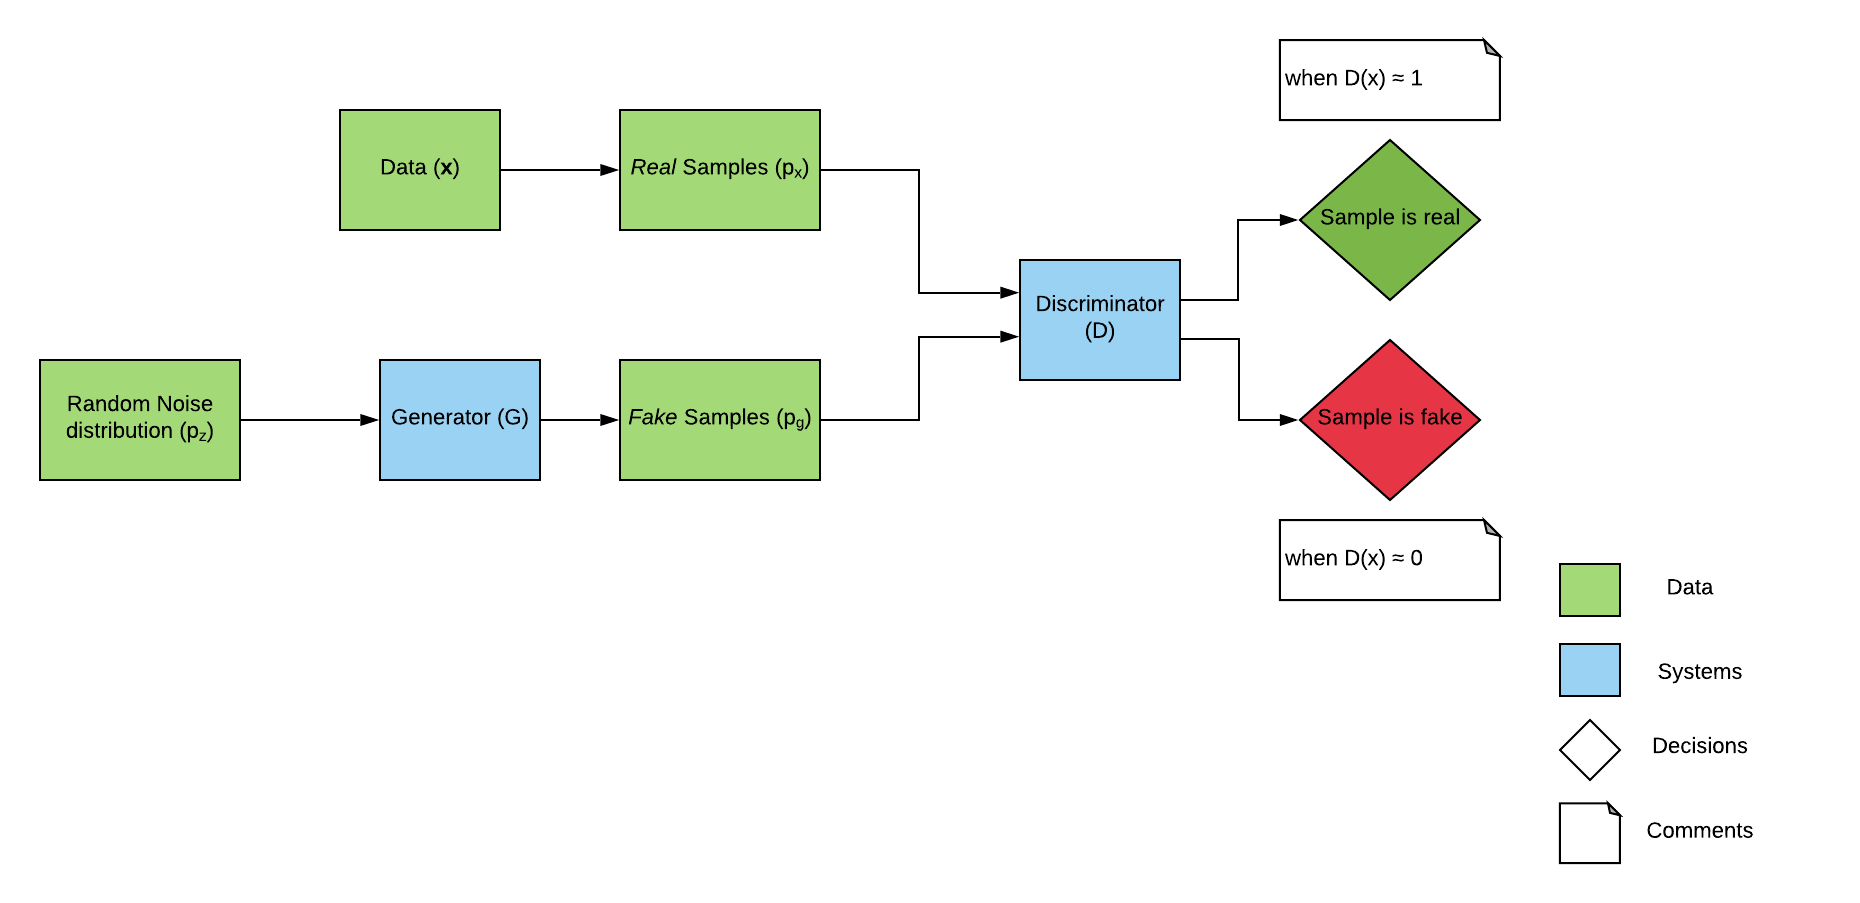
\includegraphics[scale=0.55]{figures/GAN_v4.png}
    \caption{An illustration of the general structure of a Generative Adversarial Network}
    \label{fig:gan-diagram}
\end{figure}    

As we can see in figure \ref{fig:gan-diagram}, $G$ generates samples from a random noise distribution $p_z$. We call the resulting data distribution $p_g$; $D$ is fed both data from the training set ($x$) and the output from $G$ ($p_g$), and it's task is to figure out whether any given sample comes from the data (it belongs to $p_x$) or has been generated from $G$ (it belongs to $p_g$). In layman terms, we might say that it is $D$'s job to tell \enquote{real} samples from \enquote{fake} ones.

Goodfellow et al.\cite{Goodfellow2014} explain the interplay between the two networks as a min-max game: the goal of $D$ is to maximize the likelihood of guessing correctly, while the goal of $G$ is to minimize that same likelihood (or to put it another way, $G$ wants $D$ to make more mistakes): the reason for this is that by minimizing the likelihood of $D$ guessing correctly, we are implicitly telling $G$ to generate samples as close as possible to the input data.

Simply put, the two networks are trying to out-smart each other: $D$ tries to spot the fake samples from $p_g$, while $G$ tries to improve more and more to make $D$'s job harder.

The output of $D$ is a single value between 0 and 1 expressing the network's confidence on whether a sample came from $x$: values of $D(x)$ closer to 1 tend towards assigning a sample to the input data distribution.
Ideally, this race/competition between the two networks comes to an end when the output $D(x)$ stabilizes on $D(x)=0.5$, meaning that $D$ is no longer able to tell the two distributions apart.

This also tells us that if we had infinite resources (both in  data samples and computing resources), we could train until $D(x)=0.5$ and $p_x=p_g$, giving us an output of $G$ that is indistinguishable from the input data.

One important thing to note is that we do not show $G$ any of the input data at any point: all that $G$ has access to is a random noise distribution and the error value for $D$; the Generator has to slowly shape that noise into data resembling the Discriminator's input, by using Gradient Descent.  

The process described above can be formalized in the following general equation:
\begin{equation}
 \min\limits_{G} \max\limits_{D} V(D,G)=\mathbb{E}_{x\sim p_{data}(x)}[\log{D(x)}]+\mathbb{E}_{z\sim p_z(z)}[\log{(1-D(G(z)))}] 
\end{equation} 

Since the network relies on this tight feedback loop between $D$ and $G$ to operate, one needs to pay close attention to how quickly each individual network learns.
The idea, as the authors in \cite{Goodfellow2014} point out, is to have a certain number of iterations of $D$ before we go ahead and adjust the Error for $G$. Conceptually, we might think of this as giving $D$ enough time to tell the real data from the fake data reliably (or try), before iterating $G$ to counter $D$'s current strategy.

The original paper indicates this ratio with $k$, and notes that increasing it grows the required computation significantly. In their experiments the authors used a $k$ value of 1 for performance reasons, while PassGAN defaults to a $k$ value of 10\cite{PassGAN}.

\subsubsection{PassGAN}\label{subsubsec:gans-passgan}
PassGAN is a generative adversarial network built to generate password candidates for the purposes of password cracking. In it, $G$ and $D$ compete in an attempt to generate passwords that closely mimic the real passwords fed to the network as input data.

In this section, we will go over some of the important hyper-parameters used with PassGAN and some other concepts that will become relevant is section \ref{sec:testing_and_evaluation}, where we put PassGAN to the test.

In order to train PassGAN, we use the passwords from the Libero dataset mentioned in section \ref{subsec:password_cracking}. As is common with deep neural network training, we split our data into two subsets of 80\% and 20\%: the 80\% of the passwords are used for Training, while 20\% are used for Testing. 

 The Training phase is what we covered in section \ref{subsubsec:gans}, but we did not talk about Testing in this chapter: generally speaking testing is the practice of presenting a newly-trained deep learning system with new data it has not seen before, in order to test whether the model performs as expected outside of the limited scope of the training data.

For some simpler machine learning systems like image classifiers (a deep learning system trained to recognized hand-written digits is a very common example), all image data is labelled with what they are supposed to be (\emph{e.g} the label might say what digit a particular image is supposed to be): if we split our data 80\%-20\% like we mentioned before, at the end of training we can present our network with the 20\% of data we put aside and use the labels to quantify whether it can guess as accurately as we expect. 

As an example of why Testing is needed, one of the risks associated with deep learning systems is \emph{over-fitting}: over-fitting is a phenomenon wherein the network is \enquote{over trained} so to speak, it performs amazingly on the training data but is not flexible enough to maintain that performance with real data outside the narrow scope of training. Intuitively, we might think of it as the network being hyper-focused on the minute characteristics of the training data: it works very well in that specific context but it does not scale well, the features that the network picks up on might not be abstract or general enough to apply in a general case. 

%Niels had a comment about this part, try to remember what it was.
We are discussing the testing process in some depth because there is an important difference between PassGAN and image classifiers: the testing process described above simply does not work with PassGAN.
This is because PassGAN does not simply classify existing data, it creates new and unique data with potentially unseen characteristics: because we do  not know what kind of string PassGAN will generate in advance, we cannot write labels for them. Even if we were able to do so, we think that the nature of GANs is at odds with this approach since the interplay between $G$ and $D$ provides the same sort of feedback as labels do on image classifiers.\\

%Not sure this is true, maybe in general or maybe only for FLA
This lack of an easily defined testing methodology or metrics are common among generative deep learning systems, RNNs focused on data generation have a similar issue.

Because of the reasons mentioned above, PassGAN has no built-in method for testing: instead, we have to rely on external methods to test the model's performance.
In this paper we want to test cracking performance, so we use the password candidates produced by PassGAN in rule-based password crackers: this process will be covered in more detail in section \ref{sec:testing_and_evaluation}, for now we will say that we used 20\% of our password data as the target of our cracking attempts with PassGAN and HashCat.\\% and the password candidates coming from PassGAN.\\
To clarify we followed the same testing methodology as Hitaj et  al. \cite{PassGAN}, just using different datasets for training and testing.

Another important concept to introduce is that of a \emph{Model}: we have used this term already several times, but to clarify we shall introduce it properly here.\\
A model is what results at the end of training of a neural network: in essence it is a snap-shot of all the weights and parameters present in the network, that taken together tell the network what to do with a given input. Once we load a model into a neural network we can use it to process new data, and we tests the model with our testing data to verify that it is as accurate new data as it was with the training data.

PassGAN's approach to models is rather common, and it works as follows: by default PassGAN is programmed to take a model snap-shot every 5000 iterations (called a checkpoint in the software), potentially allowing us to use a partially trained model if we so desire; if we want to use the final model, we simply choose the latest snap-shot available.\\
Models are then used when generating password candidates through sampling, where we tell PassGAN what model we would like to use for generating our passwords and how many we want. Generally we will want to use the latest model available to get the best possible results, but because we have access to snap-shots from various points in the training process we may choose to use an older, partial model in order to observe how the kinds of passwords PassGAN generates change over the course of training.

The sampling process will be explained better in section \ref{subsec:passgan-training}. As a reference, in all our tests we used the latest snap-shot/model available and we generated either 1.000.000 password candidates or 14.000.000 password candidates.
Note that the number of models available changes depending on the amount of data and the length of training: using less data for training will result in fewer iterations and thus less snap-shots available, and vice versa.

%\cleardoublepage
Shifting our discussion to the hyper-parameters used with PassGAN, they are values we can change to influence how the training is done. All of the hyper-parameters present in Hitaj et al. \cite{PassGAN} were kept the same in this paper. We will briefly touch upon some of them, explaining what they do and mentioning how they influenced our testing of PassGAN.

There are three hyper-parameters that are relevant to this discussion: the first is \emph{sequence length}, a number that defines the maximum length of password candidates generated by PassGAN; this value is set to 10.\\ 
Sequence length is important because it will influence what kind of passwords we use for testing, for the explanation of how sequence length comes into play the reader may look at section \ref{subsec:passgan-testing}.
%might be wrong: training lenght should be set by setting the maximum number of training samples in the source code.
Another important hyper-parameter is the number of total iterations, which defines for how long PassGAN should train: this number is set to $200000$, but PassGAN never reaches the last iteration during our tests: Hitaj. et al. arrived at this value after several experiments as the ideal length of training for their case, however in our paper we have a considerably smaller training dataset of around 530,000 passwords (80\% of the Libero set), so we have noticed that our training stops around iteration number 190000 or 195000 when PassGAN runs out of input data.

In hindsight we should have tried to tweak the iteration count to optimize for our particular amount of data: we don't really know if this had a negative impact on the resulting model, the extra iterations might have lead to over fitting, but we would not be able to tell as we did not have another model trained with a lower number of iterations as a term of comparison.\\
This might be seen as one of the downsides of using a generative system like a GAN: testing requires a more elaborate setup and its harder to spot problems when compared to simpler systems with built-in testing methods. 
%double checck source code to see if over-fitting is actually possible nd how iterations actually work.

The third relevant hyper-parameter is $k$, one that we have already discussed at the end of the previous section. As a reminder, $k$ is a value that determines how many iterations of $D$ happen for every iteration of $G$. In effect, it controls how quick the feedback loop between the two systems is and how fast PassGAN learns and adapts. We have not modified $k$ in our testing, but we mention it again here because we think it is key in understanding how PassGAN works. 
